\documentclass[11pt]{amsart}
\usepackage[margin=1.15in]{geometry}
\usepackage{amsmath,amssymb,amsthm}
\usepackage{booktabs}
\usepackage{tikz}
\usepackage{pgfplots}
\pgfplotsset{compat=1.17}
\usepackage[colorlinks=true,linkcolor=blue!55!black,citecolor=blue!55!black,urlcolor=blue!55!black]{hyperref}

\newtheorem{theorem}{Theorem}
\newtheorem{lemma}[theorem]{Lemma}
\newtheorem{corollary}[theorem]{Corollary}
\theoremstyle{remark}
\newtheorem{remark}[theorem]{Remark}

\newcommand{\R}{\mathbb{R}}
\newcommand{\Q}{\mathbb{Q}}
\newcommand{\gp}{\varphi}

\begin{document}

\title[Escape paths for isosceles triangles]{An improved upper bound for
Bellman's lost-in-a-forest problem in isosceles triangles}

\author{Alexander Temerev}
\address{University of Geneva, Geneva, Switzerland}
\email{alexander.temerev@unige.ch}
\thanks{The computations, the verification scripts, and the initial draft of
this manuscript were produced with the assistance of Claude (Anthropic).
Verification code is provided as ancillary files.}

\date{July 21, 2026}

\begin{abstract}
We prove a new upper bound for the escape length of isosceles triangles in
Bellman's lost-in-a-forest problem, on an entire interval of base angles
inside the unsolved range.  We construct an explicit piecewise-polynomial
family of three-segment paths $S(u)$, $u=\tan(\beta/2)$, with
isosceles-trapezoidal convex hull (``staples''), and prove that $S(u)$
escapes the triangle $T(\beta)$ with unit legs and base angle $\beta$, and is
strictly shorter than every escaping square path, for all
$\beta\in[31.08^\circ,42.16^\circ]$; on $[31.50^\circ,42.16^\circ]$ it is also
strictly shorter than the diameter, the scaled Zalgaller caliper, and the
Besicovitch--Movshovich zee.  This interval strictly contains
$(32.36^\circ,41.34^\circ)$, the range on which Ward's square path was the
shortest known candidate, so the square path is removed from the frontier
everywhere, and the trapezoidal improvement Ward reported numerically in 2008
becomes a theorem, with the enlarged range he predicted certified at both
ends.  The proofs eliminate the continuum of positions and headings exactly:
escape from a triangle reduces, via the planar case of a containment theorem
of Lutwak, to the containment of a disk in an explicit Minkowski sum, and
every resulting inequality is a rational-polynomial sign condition verified
by exact Sturm certificates.  At the type example, the golden gnomon (apex
$108^\circ$), the bound reads
$\ell(T)\le\frac{3751558+2\sqrt{20693661817348}}{10^{7}}=1.2849616\ldots$
against Ward's $1.2934740\ldots$, with the closed-form bracket
$\tfrac{3}{10}\sqrt{25-5\sqrt5}\le\ell(T)$.  Optimality is not claimed.
\end{abstract}

\maketitle

\section{Introduction}

Bellman \cite{bellman1956} asked for the shortest walk guaranteed to leave a
forest of known shape when the hiker knows neither their position nor their
heading.  Formally, a rectifiable path $P\subset\R^2$ is an \emph{escape
path} for a compact convex region $T$ if no congruent copy of $P$ lies in
$\operatorname{int}T$; the \emph{escape length} $\ell(T)$ is the infimum of
the lengths of such paths \cite{finchwetzel2004}.

\subsection*{Seventy years of improvements}
Progress has come one shape --- and one mechanism --- at a time.  Gross
\cite{gross1955} settled the disk: the diameter walk is optimal.  Isbell
\cite{isbell1957}, completed by Joris \cite{joris1980}, settled the
half-plane at known distance.  Zalgaller \cite{zalgaller1961} settled the
infinite strip with the \emph{caliper}, of length $\zeta=2.2782916\ldots$ per
unit width (see also \cite{adhikaripitman1989,chan2003}).  Gerriets and Poole
\cite{gerrietspoole1974} proved that all \emph{fat} regions --- those
containing a $60^\circ$ rhombus on a diameter --- are escaped optimally by a
diameter segment.  Besicovitch's zigzag \cite{besicovitch1965} for the
equilateral triangle was proven optimal by Coulton and Movshovich
\cite{coultonmovshovich2006}, and Movshovich \cite{movshovich2012} extended
the optimality of the associated \emph{zee} zigzags to all isosceles
triangles with base angles in $[45^\circ,60^\circ]$ (see also
\cite{movshovichwetzel2011}).

\subsection*{Why triangles}
The solved cases sort into two one-dimensional mechanisms.  Fat regions are
governed by the \emph{diameter}: the longest chord already escapes
optimally.  Lean regions are governed by \emph{width}: an arc of width $w$
cannot be hidden in a region of width $w$, so the scaled caliper gives
$\ell(K)\le\zeta\,w(K)$, exact for the strip and asymptotically right for
long thin regions.  Triangles belong to neither regime: a triangle is never
fat (its diameter is one of its sides, and the rhombus needs room on both
sides of that chord), and it is lean only in the limit of small base angle.
They are thus the simplest forests squeezed strictly between the two solved
mechanisms, and each solved triangular case has required a genuinely new
path: the zigzags of Besicovitch and Movshovich on
$[45^\circ,60^\circ]$.  Below $45^\circ$ the problem is open, and the
isosceles family $T(\beta)$ --- unit legs, base angles $\beta$, base
$2\cos\beta$ --- is its standard laboratory.

Ward \cite{ward2008} explored this open range numerically.  He compared the
scaled caliper, the zee, the diameter, and a fourth candidate, the
\emph{square path} (three sides of a square), and found the square path
shortest among the four for $32.36^\circ<\beta<41.34^\circ$; from this he
concluded (his Proposition~15) that ``there exists at least one more type of
solution for bounded forests.''  He then recorded the following, which we
quote in full since it is the subject of this paper:
\begin{quote}
``Some numerical experiments indicate that the results for the square
can be improved slightly by increasing the lower base to form a path
with an isosceles trapezoidal convex hull. This leads to shorter path
lengths and a slightly larger range over which the path surpasses
Zalgaller and Besicovitch.'' \cite[p.~49]{ward2008}
\end{quote}
He published no coordinates or lengths for this improvement.  Gibbs
\cite{gibbs2016}, using an uncertified Monte-Carlo search, later placed a
``trapezium'' phase near base angles $38^\circ$--$42^\circ$.  Recent work of
Deng \cite{deng2025,deng2026} formulates the general problem as a
boundary-intersection problem and studies finite traveling-salesman
discretizations.  Our aim is complementary: for triangular forests the
continuum of positions and headings can be eliminated \emph{exactly} --- a
path escapes if and only if one explicit Minkowski sum contains a disk
(Section~\ref{sec:criterion}) --- and candidate paths then admit finite,
checkable certificates.  No sampled positions or orientations occur in any
proof below.

\subsection*{Main result}
A \emph{staple} is a three-segment path whose four vertices
$(\pm b,0),(\pm a,c)$ form an isosceles trapezoid: a bar of length $2b$ with
two equal legs attached at equal obtuse angles
(Figure~\ref{fig:family}).  Ward's square path is the case $a=b$, $c=2b$;
releasing the right angles is what saves length.

\begin{theorem}\label{thm:interval}
Let $u=\tan(\beta/2)$, and let $S(u)$ be the staple whose parameters
$a(u),b(u),c(u)$ are the explicit rational polynomials of
Section~\ref{sec:interval} (degrees at most $6$; $51$ rational coefficients
in total, listed in the ancillary file
\texttt{interval\_construction.json}).  Then for every
$u\in[0.278,\,0.3855]$, that is for every base angle
$\beta=2\arctan u\in[31.0719^\circ,\,42.1633^\circ]$:
\begin{enumerate}
\item[(i)] $S(u)$ is an escape path for $T(\beta)$;
\item[(ii)] $|S(u)| < 3s$ for every square path of side $s$ that escapes
$T(\beta)$ --- in particular $|S(u)|$ is strictly smaller than Ward's
square-path length in both of its regimes;
\item[(iii)] $|S(u)|$ is strictly smaller than the zee length
$\frac{6\sin\beta\cos\beta}{\sqrt{1+8\sin^2\beta}}$ and the diameter
$2\cos\beta$; and for $u\ge 0.282$ (i.e.\ $\beta\ge31.4969^\circ$) also
strictly smaller than the caliper length $\zeta\sin\beta$.
\end{enumerate}
\end{theorem}

\begin{corollary}[Ward's enlargement, certified]\label{cor:trio}
For every base angle
$\beta\in[31.50^\circ,\,42.16^\circ]\supsetneq(32.36^\circ,41.34^\circ)$,
the staple $S(u(\beta))$ is an escape path for $T(\beta)$ strictly shorter
than each of the four candidates compared by Ward: the diameter, the scaled
Zalgaller caliper, the Besicovitch--Movshovich zee, and every escaping
square path.
\end{corollary}

Figure~\ref{fig:curves} shows the five length curves.  Two features are the
content of Theorem~\ref{thm:interval}: the staple curve lies strictly below
the square-path curve across a band that covers Ward's entire square-path
range, so the square path is now nowhere the best known candidate; and it
lies below all four competitors on $[31.50^\circ,42.16^\circ]$, certifying
the enlargement Ward predicted --- at both ends.

\begin{figure}[t]
\centering
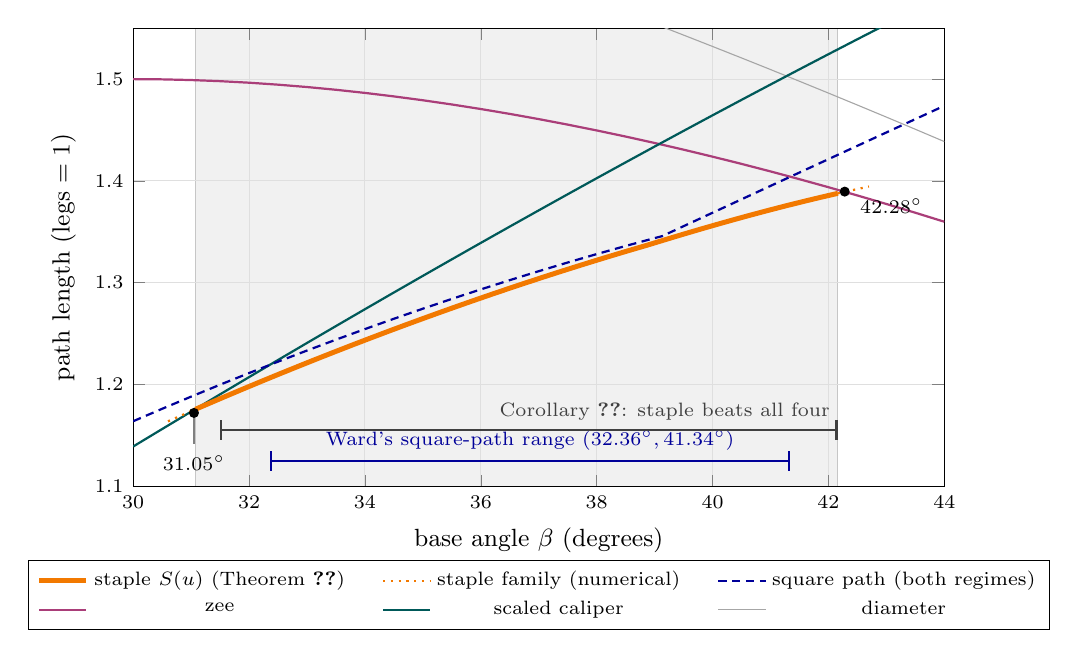
\begin{tikzpicture}
\begin{axis}[width=0.98\textwidth, height=7.4cm, set layers,
  xlabel={base angle $\beta$ (degrees)}, ylabel={path length (legs $=1$)},
  xmin=30, xmax=44, ymin=1.10, ymax=1.55,
  legend style={at={(0.5,-0.16)}, anchor=north, legend columns=3,
                font=\scriptsize, /tikz/every even column/.append style={column sep=0.4cm}},
  tick label style={font=\scriptsize}, label style={font=\small},
  grid=major, grid style={gray!25}]
% certified band: on the background layer, so the grid stays visible
\begin{pgfonlayer}{axis background}
\fill[gray!11] (axis cs:31.0719,1.10) rectangle (axis cs:42.1633,1.55);
\draw[gray!45, thin] (axis cs:31.0719,1.10) -- (axis cs:31.0719,1.55);
\draw[gray!45, thin] (axis cs:42.1633,1.10) -- (axis cs:42.1633,1.55);
\end{pgfonlayer}
% legend in priority order (independent of drawing order)
\addlegendimage{orange!95!black, line width=1.8pt}
\addlegendentry{staple $S(u)$ (Theorem~\ref{thm:interval})}
\addlegendimage{orange!95!black, line width=0.8pt, dotted}
\addlegendentry{staple family (numerical)}
\addlegendimage{blue!60!black, thick, densely dashed}
\addlegendentry{square path (both regimes)}
\addlegendimage{magenta!65!black, thick}
\addlegendentry{zee}
\addlegendimage{teal!70!black, thick}
\addlegendentry{scaled caliper}
\addlegendimage{gray!70, thin}
\addlegendentry{diameter}
% curves
\addplot[gray!70, thin, forget plot] coordinates {
(30.000,1.73205) (31.000,1.71433) (32.000,1.69610) (33.000,1.67734)
(34.000,1.65808) (35.000,1.63830) (36.000,1.61803) (37.000,1.59727)
(38.000,1.57602) (39.000,1.55429) (39.250,1.54879) (39.500,1.54325)
(39.750,1.53768) (40.000,1.53209) (40.500,1.52081) (41.000,1.50942)
(41.500,1.49791) (42.000,1.48629) (42.500,1.47455) (43.000,1.46271)
(43.500,1.45075) (44.000,1.43868)};
\addplot[magenta!65!black, thick, forget plot] coordinates {
(30.000,1.50000) (30.500,1.49977) (31.000,1.49910) (31.500,1.49800)
(32.000,1.49649) (32.500,1.49456) (33.000,1.49224) (33.500,1.48954)
(34.000,1.48647) (34.500,1.48303) (35.000,1.47924) (35.500,1.47511)
(36.000,1.47064) (36.500,1.46585) (37.000,1.46074) (37.500,1.45532)
(38.000,1.44960) (38.500,1.44359) (39.000,1.43729) (39.500,1.43071)
(40.000,1.42385) (40.500,1.41674) (41.000,1.40936) (41.500,1.40172)
(42.000,1.39384) (42.500,1.38572) (43.000,1.37736) (43.500,1.36876)
(44.000,1.35994)};
\addplot[teal!70!black, thick, forget plot] coordinates {
(30.000,1.13915) (30.500,1.15632) (31.000,1.17341) (31.500,1.19040)
(32.000,1.20731) (32.500,1.22413) (33.000,1.24085) (33.500,1.25747)
(34.000,1.27400) (34.500,1.29044) (35.000,1.30677) (35.500,1.32301)
(36.000,1.33915) (36.500,1.35518) (37.000,1.37111) (37.500,1.38694)
(38.000,1.40266) (38.500,1.41827) (39.000,1.43378) (39.500,1.44917)
(40.000,1.46446) (40.500,1.47963) (41.000,1.49469) (41.500,1.50964)
(42.000,1.52447) (42.500,1.53919) (43.000,1.55379)};
\addplot[blue!60!black, thick, densely dashed, forget plot] coordinates {
(30.000,1.16399) (30.500,1.17620) (31.000,1.18816) (31.500,1.19986)
(32.000,1.21130) (32.500,1.22249) (33.000,1.23342) (33.500,1.24409)
(34.000,1.25449) (34.500,1.26464) (35.000,1.27452) (35.500,1.28413)
(36.000,1.29347) (36.500,1.30255) (37.000,1.31136) (37.500,1.31989)
(38.000,1.32815) (38.500,1.33614) (39.000,1.34385) (39.132,1.34581)
(39.250,1.34896) (39.500,1.35557) (40.000,1.36877) (40.500,1.38195)
(41.000,1.39511) (41.500,1.40826) (42.000,1.42139) (42.500,1.43451)
(43.000,1.44762) (43.500,1.46072) (44.000,1.47382)};
\addplot[orange!95!black, line width=1.8pt, forget plot] coordinates {
(31.072,1.17566) (31.372,1.18301) (31.672,1.19028) (31.972,1.19745)
(32.272,1.20454) (32.572,1.21153) (32.872,1.21844) (33.172,1.22526)
(33.472,1.23198) (33.772,1.23862) (34.072,1.24516) (34.372,1.25161)
(34.672,1.25797) (34.972,1.26423) (35.272,1.27040) (35.572,1.27648)
(35.872,1.28246) (36.172,1.28835) (36.472,1.29414) (36.772,1.29983)
(37.072,1.30543) (37.372,1.31093) (37.672,1.31632) (37.972,1.32162)
(38.272,1.32682) (38.572,1.33192) (38.872,1.33691) (39.172,1.34213)
(39.472,1.34728) (39.772,1.35231) (40.072,1.35723) (40.372,1.36203)
(40.672,1.36670) (40.972,1.37124) (41.272,1.37564) (41.572,1.37989)
(41.872,1.38399) (42.163,1.38782)};
\addplot[orange!95!black, line width=0.8pt, dotted, forget plot] coordinates {
(30.600,1.16388) (30.800,1.16887) (31.000,1.17386) (31.072,1.17566)};
\addplot[orange!95!black, line width=0.8pt, dotted, forget plot] coordinates {
(42.163,1.38782) (42.300,1.38957) (42.500,1.39204) (42.700,1.39448)};
% crossings (numerical, Section 6)
\addplot[only marks, mark=*, mark size=1.6pt, black, forget plot] coordinates {
(31.049,1.17215) (42.281,1.38951)};
\draw[gray, thin] (axis cs:31.049,1.168) -- (axis cs:31.049,1.142);
\node[font=\scriptsize, anchor=north] at (axis cs:31.049,1.140) {$31.05^\circ$};
\node[font=\scriptsize, anchor=west] at (axis cs:42.38,1.375) {$42.28^\circ$};
% Ward's interval and the certified interval
\draw[blue!60!black, |-|, thick] (axis cs:32.36,1.125) -- (axis cs:41.34,1.125)
  node[midway, above, font=\scriptsize] {Ward's square-path range $(32.36^\circ,41.34^\circ)$};
\draw[black!75, |-|, thick] (axis cs:31.50,1.155) -- (axis cs:42.16,1.155)
  node[pos=0.72, above, font=\scriptsize, black!75] {Corollary~\ref{cor:trio}: staple beats all four};
\end{axis}
\end{tikzpicture}
\caption{The five candidate lengths against the base angle $\beta$.  The
shaded band $[31.07^\circ,42.16^\circ]$ is the certified domain of
Theorem~\ref{thm:interval}: there the staple $S(u)$ (thick) escapes and lies
strictly below the square-path curve, whose two regimes meet in the visible
kink at $\beta_0=39.132^\circ$.  On the marked subinterval it lies below all
four competitors.  Dotted continuations and the two crossing points at
$31.05^\circ$ and $42.28^\circ$ are numerical (Section~\ref{sec:numerics});
everything else in the band is proved.}
\label{fig:curves}
\end{figure}

\subsection*{The type example}
At a single pleasant triangle the bound becomes a closed-form statement.
The \emph{golden gnomon} is the isosceles triangle with unit legs, apex
$108^\circ$ (base angles $36^\circ$), and base $\gp=(1+\sqrt5)/2$.

\begin{theorem}\label{thm:gnomon}
Let $T$ be the golden gnomon, and let $S$ be the polygonal path through
\[
\left(-\frac{2430971}{10^{7}},\frac{4515022}{10^{7}}\right),\quad
\left(-\frac{1875779}{10^{7}},0\right),\quad
\left( \frac{1875779}{10^{7}},0\right),\quad
\left( \frac{2430971}{10^{7}},\frac{4515022}{10^{7}}\right).
\]
Then $S$ escapes $T$, and
\[
 \ell(T)\le |S|
 =\frac{3751558+2\sqrt{20693661817348}}{10^{7}}
 =1.28496153349145\ldots <1.284962 .
\]
In particular $|S|$ is smaller than Ward's square-path length
$1.293473869\ldots$, by $8.512\times10^{-3}$.
\end{theorem}

\begin{corollary}[a rigorous bracket]\label{cor:bracket}
For the golden gnomon,
\[
 \frac{3}{10}\sqrt{25-5\sqrt5}
 \;=\;1.115244103\ldots
 \;\le\;\ell(T)\;<\;1.284962.
\]
\end{corollary}

Figure~\ref{fig:panels} compares the path of Theorem~\ref{thm:gnomon} with
the four standard candidates at the gnomon.  Sections
\ref{sec:criterion}--\ref{sec:gnomon} contain the proofs;
Section~\ref{sec:numerics} separates out the numerical evidence (stationary
staples, family crossings) that guided the constructions but enters no
proof.  We emphasize what is \emph{not} claimed: optimality of the staple,
within its family or otherwise.

\begin{figure}[t]
\centering
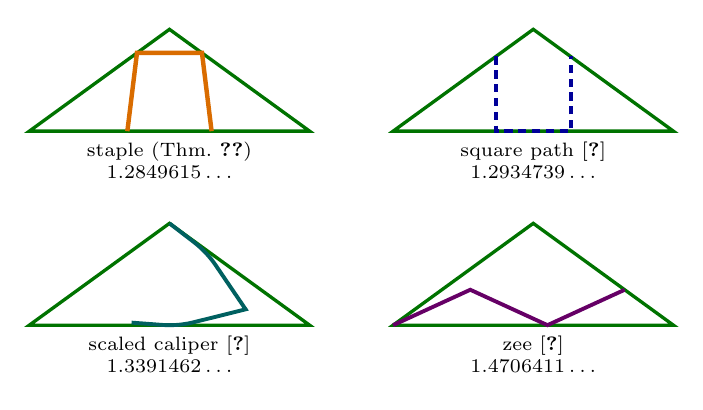
\begin{tikzpicture}[scale=2.2]
\newcommand{\gnomon}{\draw[very thick,green!45!black]
 (-0.80902,0) -- (0.80902,0) -- (0,0.58779) -- cycle;}
\begin{scope}[shift={(-1.05,0)}]
\gnomon
\draw[line width=1.6pt,orange!85!black]
 (0.24310,0) -- (0.18758,0.45150) -- (-0.18758,0.45150) -- (-0.24310,0);
\node[font=\scriptsize,align=center] at (0,-0.17)
 {staple (Thm.~\ref{thm:gnomon})\\ $1.2849615\ldots$};
\end{scope}
\begin{scope}[shift={(1.05,0)}]
\gnomon
\draw[line width=1.4pt,densely dashed,blue!60!black]
 (-0.21558,0.43116) -- (-0.21558,0) -- (0.21558,0) -- (0.21558,0.43116);
\node[font=\scriptsize,align=center] at (0,-0.17)
 {square path \cite{ward2008}\\ $1.2934739\ldots$};
\end{scope}
\begin{scope}[shift={(-1.05,-1.12)}]
\gnomon
\draw[line width=1.4pt,teal!75!black] plot coordinates {
(0.00000,0.58779) (0.13915,0.48094) (0.14360,0.47749) (0.14802,0.47399)
(0.15241,0.47045) (0.15676,0.46687) (0.16108,0.46325) (0.16537,0.45958)
(0.16961,0.45588) (0.17383,0.45213) (0.17800,0.44835) (0.18214,0.44452)
(0.18625,0.44066) (0.19031,0.43675) (0.19434,0.43281) (0.19833,0.42883)
(0.20228,0.42481) (0.20620,0.42075) (0.21007,0.41666) (0.21391,0.41252)
(0.21770,0.40836) (0.22146,0.40415) (0.22517,0.39991) (0.22885,0.39564)
(0.23248,0.39132) (0.23607,0.38698) (0.23962,0.38260) (0.24312,0.37819)
(0.24659,0.37374) (0.25001,0.36926) (0.25339,0.36475) (0.25672,0.36020)
(0.26002,0.35562) (0.26326,0.35102) (0.26647,0.34638) (0.43970,0.09158)
(0.14209,0.01743) (0.13662,0.01610) (0.13113,0.01481) (0.12563,0.01358)
(0.12011,0.01240) (0.11459,0.01128) (0.10906,0.01021) (0.10351,0.00919)
(0.09796,0.00822) (0.09239,0.00731) (0.08682,0.00645) (0.08124,0.00564)
(0.07566,0.00489) (0.07006,0.00419) (0.06446,0.00355) (0.05886,0.00295)
(0.05325,0.00242) (0.04763,0.00193) (0.04201,0.00150) (0.03638,0.00113)
(0.03076,0.00081) (0.02512,0.00054) (0.01949,0.00032) (0.01386,0.00016)
(0.00822,0.00006) (0.00258,0.00001) (-0.00305,0.00001) (-0.00869,0.00006)
(-0.01433,0.00017) (-0.01996,0.00034) (-0.02559,0.00056) (-0.03122,0.00083)
(-0.03685,0.00116) (-0.04248,0.00154) (-0.04388,0.00164) (-0.21883,0.01474)};
\node[font=\scriptsize,align=center] at (0,-0.17)
 {scaled caliper \cite{zalgaller1961}\\ $1.3391462\ldots$};
\end{scope}
\begin{scope}[shift={(1.05,-1.12)}]
\gnomon
\draw[line width=1.4pt,violet!80!black]
 (-0.80902,0) -- (-0.36346,0.20442) -- (0.08210,0) -- (0.52766,0.20442);
\node[font=\scriptsize,align=center] at (0,-0.17)
 {zee \cite{movshovich2012}\\ $1.4706411\ldots$};
\end{scope}
\end{tikzpicture}
\caption{The four candidates at the golden gnomon (legs $1$, apex
$108^\circ$, diameter $1.6180340$), each drawn at a critical placement: each
path's hull fits $T$ only in touching position.  The staple of
Theorem~\ref{thm:gnomon} achieves criticality at the smallest length.}
\label{fig:panels}
\end{figure}

\section{The escape criterion}\label{sec:criterion}

Throughout, $h_C(u)=\sup_{x\in C}\langle x,u\rangle$ denotes the support
function of a compact convex set $C$, and $R_\theta$ the rotation of
$\R^2$ by angle $\theta$. We use two standard facts: $h_{C\oplus D}=h_C+h_D$
for the Minkowski sum, and $h_{RC}(u)=h_C(R^{-1}u)$.

\begin{lemma}[hull reduction]\label{lem:hull}
A path $P$ is an escape path for a convex region $T$ if and only if for
every rotation $\theta$ there is no translation $t$ with
$R_\theta\operatorname{conv}(P)+t\subset\operatorname{int}T$.
\end{lemma}

\begin{proof}
A placed copy of $P$ lies in the open convex set
$\operatorname{int}T$ if and only if its convex hull does; rigid
motions factor as a rotation followed by a translation. (If a placed
copy is not contained in the interior, the connected path starting
inside must meet $\partial T$, i.e.\ the hiker escapes; cf.\
\cite{finchwetzel2004}.)
\end{proof}

\begin{lemma}[fit criterion for triangles]\label{lem:fit}
Let $T=\{x:\langle n_i,x\rangle\le t_i,\ i=1,2,3\}$ be a triangle with
unit outward normals $n_i$ and side lengths $s_i$, so that
$\sum_i s_i n_i=0$ and $\sum_i s_i t_i = 2\operatorname{Area}(T)$.
For a compact convex $C$ there exists a translation $t$ with
$C+t\subseteq T$ if and only if
\[
s_1 h_C(n_1)+s_2 h_C(n_2)+s_3 h_C(n_3)\;\le\;2\operatorname{Area}(T).
\]
\end{lemma}

Since $\sum_i s_i\,h_C(n_i)=2V(C,T)$, twice the mixed area, the
criterion reads: \emph{$C$ translates into $T$ if and only if
$V(C,T)\le V(T,T)=\operatorname{Area}(T)$}. In this mixed-volume form
(for simplices in all dimensions) the criterion is a result of Lutwak
\cite[Prop., p.~230 and the remark following Cor.~3]{lutwak1998}, with
ancestry in Weil's characterization of translative containment
\cite{weil1974}. We include the short linear-programming proof both to
keep the note self-contained and because its sufficiency half produces
the explicit feasible translations used in our certificates.  We have not
found this finite disk-containment specialization in the escape-path
literature.

\begin{proof}
$C+t\subseteq T$ is equivalent to the linear system
$\langle n_i,t\rangle\le c_i:=t_i-h_C(n_i)$, $i=1,2,3$.

\emph{Necessity.} If $t$ solves the system then
$0=\langle\sum_i s_i n_i,t\rangle\le\sum_i s_i c_i$, which rearranges to
the stated inequality.

\emph{Sufficiency.} Suppose
$\lambda:=\bigl(\sum_i s_i c_i\bigr)/\bigl(2\operatorname{Area}(T)\bigr)\ge0$.
The affine system $\langle n_i,t_0\rangle=c_i-\lambda t_i$ ($i=1,2,3$;
three equations in two unknowns) is solvable: the unique linear
dependency among the rows $n_i$ has coefficients $s_i$, and
$\sum_i s_i(c_i-\lambda t_i)=\sum_i s_i c_i-\lambda\cdot2\operatorname{Area}(T)=0$
is precisely its compatibility condition. For this $t_0$,
\[
\{t:\langle n_i,t\rangle\le c_i\}\;=\;\lambda T+t_0\;\neq\;\emptyset .\qedhere
\]
\end{proof}

Note the geometric content of sufficiency: \emph{the set of admissible
translations is itself a homothet of the triangle}, of ratio $\lambda$.

\begin{corollary}[Minkowski criterion]\label{cor:mink}
With $T$, $n_i=(\cos\alpha_i,\sin\alpha_i)$, $s_i$ as above, a path $P$
with $H=\operatorname{conv}(P)$ is an escape path for $T$ if and only if
the Minkowski sum
\[
W\;:=\;s_1\,R_{-\alpha_1}H\;\oplus\;s_2\,R_{-\alpha_2}H\;\oplus\;s_3\,R_{-\alpha_3}H
\]
contains the closed disk of radius $2\operatorname{Area}(T)$ centered at
the origin.  If $H$ is a polygon, then so is $W$.
\end{corollary}

\begin{proof}
By Lemmas \ref{lem:hull}--\ref{lem:fit}, $P$ escapes iff for all
$\theta$,
$\sum_i s_i\,h_{R_\theta H}(n_i)\ge 2\operatorname{Area}(T)$
(the closed inequality: a hull that can only be translated to touch
$\partial T$ still reaches the boundary). Writing
$h_{R_\theta H}(n_i)=h_H(R_{-\theta}u(\alpha_i))=h_{R_{-\alpha_i}H}(u(-\theta))$
with $u(\psi)=(\cos\psi,\sin\psi)$ and summing,
$\sum_i s_i h_{R_\theta H}(n_i)=h_W(u(-\theta))$. The condition
$h_W(u)\ge 2\operatorname{Area}(T)$ for every unit $u$ is equivalent to
$W\supseteq \overline{D}(0,2\operatorname{Area}(T))$.
\end{proof}

\begin{remark}\label{rem:edgenormals}
Two computational forms of the inclusion are used below. For a fixed
triangle, $W$ is an explicit polygon and the inclusion is a list of
edge-distance inequalities (Section~\ref{sec:gnomon} and
Figure~\ref{fig:mink}). For a one-parameter family it is more convenient to
avoid tracking the boundary of $W$: a convex polygon is the intersection of
its edge half-planes, and every edge normal of a Minkowski sum is an edge
normal of one of the summands, so it suffices to verify
$h_W(\nu)\ge 2\operatorname{Area}(T)\cdot|\nu|$ for the twelve candidate
directions $\nu=R_{-\alpha_i}g$, with $g$ ranging over the four edge normals
of $H$ --- and $h_W(\nu)$ may be replaced by any convenient lower bound,
e.g.\ by evaluating each summand's support at a fixed vertex
(Section~\ref{sec:interval}).
\end{remark}

\begin{remark}
For the unit equilateral triangle the criterion reads: a path escapes iff
the Minkowski sum of three copies of its hull rotated by
$0^\circ,120^\circ,240^\circ$ contains the disk of radius
$2\operatorname{Area}=\tfrac{\sqrt3}{2}$. Besicovitch's zigzag
\cite{besicovitch1965,coultonmovshovich2006} is exactly critical in this
sense: its Minkowski sum circumscribes that disk.
\end{remark}

\section{Proof of Theorem \ref{thm:interval}}\label{sec:interval}

Parametrize by $u=\tan(\beta/2)$, so that $\sin\beta=\frac{2u}{1+u^2}$ and
$\cos\beta=\frac{1-u^2}{1+u^2}$ are rational functions of $u$.  All triangle
data --- normals, side lengths, the rotations of Corollary~\ref{cor:mink},
the disk radius $2\operatorname{Area}=\sin2\beta$ --- are then rational in
$u$, and for a staple whose parameters $a,b,c$ are \emph{polynomials} in $u$
with rational coefficients, every certificate of
Remark~\ref{rem:edgenormals}, after clearing the (positive) denominators and
squaring away the (sign-certified) square roots, is the strict positivity of
a polynomial in $\Q[u]$ on a rational interval --- decidable by Sturm's
theorem in exact integer arithmetic.

\subsection{The construction}
The ancillary file \texttt{interval\_construction.json} defines three
polynomial triples $(a_i,b_i,c_i)\in\Q[u]^3$, of degrees $6$, $2$, and $6$
on the respective pieces
\[
[0.278,\,0.3530],\qquad [0.3530,\,0.353399],\qquad [0.353399,\,0.3855],
\]
and $S(u)$ is the path through
$(-a_i(u),c_i(u)),\,(-b_i(u),0),\,(b_i(u),0),\,(a_i(u),c_i(u))$.
All $51$ coefficients are rational numbers; the machine-readable file is
part of the theorem statement, and the verification script reads it afresh
and certifies $a_i,b_i,c_i>0$ together with every inequality used below.
Figure~\ref{fig:family} shows the family at three angles.  (The two interior
breakpoints track a change in the contact pattern of the optimal staple; see
Section~\ref{sec:numerics}.)

\begin{figure}[t]
\centering
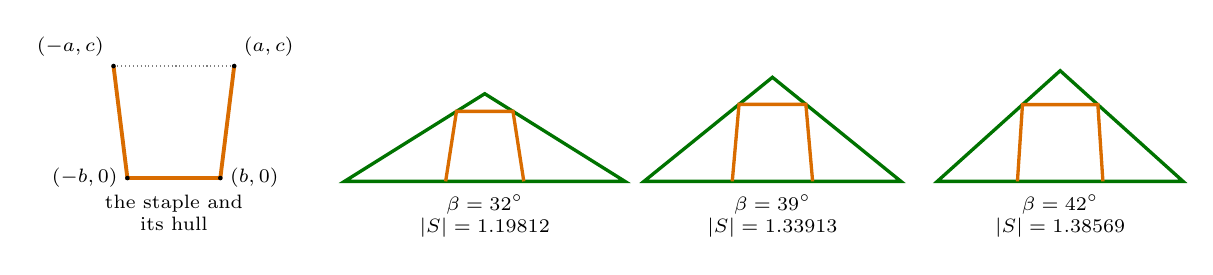
\begin{tikzpicture}[scale=2.1]
\begin{scope}[shift={(-2.75,0.02)}]
\draw[densely dotted,gray] (-0.365,0.6773) -- (0.365,0.6773);
\draw[line width=1.4pt,orange!85!black]
 (-0.365,0.6773) -- (-0.281,0) -- (0.281,0) -- (0.365,0.6773);
\fill[black] (-0.365,0.6773) circle (0.014) node[above left,font=\scriptsize] {$(-a,c)$};
\fill[black] (0.365,0.6773) circle (0.014) node[above right,font=\scriptsize] {$(a,c)$};
\fill[black] (-0.281,0) circle (0.014) node[left,font=\scriptsize] {$(-b,0)$};
\fill[black] (0.281,0) circle (0.014) node[right,font=\scriptsize] {$(b,0)$};
\node[font=\scriptsize,align=center] at (0,-0.21) {the staple and\\ its hull};
\end{scope}
\begin{scope}[shift={(-0.87,0)}]
\draw[very thick,green!45!black] (-0.84805,0) -- (0.84805,0) -- (0,0.52992) -- cycle;
\draw[line width=1.2pt,orange!85!black]
 (0.23631,0) -- (0.17087,0.42315) -- (-0.17087,0.42315) -- (-0.23631,0);
\node[font=\scriptsize,align=center] at (0,-0.21) {$\beta=32^\circ$\\ $|S|=1.19812$};
\end{scope}
\begin{scope}[shift={(0.87,0)}]
\draw[very thick,green!45!black] (-0.77715,0) -- (0.77715,0) -- (0,0.62932) -- cycle;
\draw[line width=1.2pt,orange!85!black]
 (0.24298,0) -- (0.20207,0.46569) -- (-0.20207,0.46569) -- (-0.24298,0);
\node[font=\scriptsize,align=center] at (0,-0.21) {$\beta=39^\circ$\\ $|S|=1.33913$};
\end{scope}
\begin{scope}[shift={(2.61,0)}]
\draw[very thick,green!45!black] (-0.74314,0) -- (0.74314,0) -- (0,0.66913) -- cycle;
\draw[line width=1.2pt,orange!85!black]
 (0.25843,0) -- (0.22794,0.46390) -- (-0.22794,0.46390) -- (-0.25843,0);
\node[font=\scriptsize,align=center] at (0,-0.21) {$\beta=42^\circ$\\ $|S|=1.38569$};
\end{scope}
\end{tikzpicture}
\caption{Left: a staple and its trapezoidal hull.  Right: the certified
family $S(u)$ inside $T(\beta)$ at $\beta=32^\circ$, $39^\circ$,
$42^\circ$, each at a critical placement (the hull fits only in touching
position).}
\label{fig:family}
\end{figure}

\subsection{Eliminating square paths}
\begin{lemma}[square paths from inscribed squares]\label{lem:square}
Fix $\beta$ and suppose some square $Q_0$ of side $s_0$ satisfies
$Q_0\subseteq T(\beta)$. Then every square path of side $s<s_0$ fails
to escape $T(\beta)$; consequently every escaping square path has
length $\ge 3s_0$.
\end{lemma}

\begin{proof}
The hull of a square path of side $s$ is the full square. Shrinking
$Q_0$ about its center by the factor $s/s_0<1$ places a congruent copy
of that hull in $\operatorname{int}Q_0\subseteq\operatorname{int}T(\beta)$.
\end{proof}

The two inscribed squares we use are Ward's, in exact form
(Figure~\ref{fig:squares}): the base-aligned square of side
\[
s_A=\frac{2\sin\beta\cos\beta}{\sin\beta+2\cos\beta},
\]
with both bottom corners on the base and both top corners on the legs, and
the leg-aligned square of side
\[
s_B=\frac{\sin\beta}{\sin\beta+\cos\beta},
\]
with one full side on a leg, its far corner \emph{at the apex}, and one
corner on the base.  The stated incidences are polynomial identities in
$u$; the remaining vertex--halfplane constraints are certified by Sturm
checks.  Ward's two square-path formulas $3s_A$ and $3s_B$ exchange at the
root $\beta_0=39.1320\ldots^\circ$ of
$\sin\beta\,(2\cos\beta-1)=2\cos\beta\,(1-\cos\beta)$ (his ``approximately
$39.1^\circ$''), the kink visible in Figure~\ref{fig:curves}.

\begin{figure}[t]
\centering
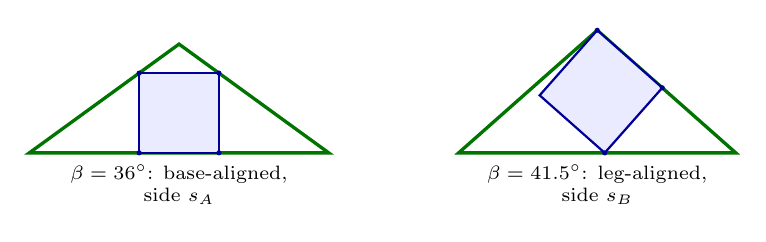
\begin{tikzpicture}[scale=2.35]
\begin{scope}[shift={(-1.13,0)}]
\draw[very thick,green!45!black] (-0.80902,0) -- (0.80902,0) -- (0,0.58779) -- cycle;
\fill[blue!8] (-0.21558,0) rectangle (0.21558,0.43116);
\draw[thick,blue!60!black] (-0.21558,0) rectangle (0.21558,0.43116);
\foreach \p in {(-0.21558,0),(0.21558,0),(0.21558,0.43116),(-0.21558,0.43116)}
  \fill[blue!60!black] \p circle (0.014);
\node[font=\scriptsize,align=center] at (0,-0.17)
 {$\beta=36^\circ$: base-aligned,\\ side $s_A$};
\end{scope}
\begin{scope}[shift={(1.13,0)}]
\draw[very thick,green!45!black] (-0.74896,0) -- (0.74896,0) -- (0,0.66262) -- cycle;
\fill[blue!8] (0.35157,0.35157) -- (0.00000,0.66262) -- (-0.31105,0.31105)
 -- (0.04053,0.00000) -- cycle;
\draw[thick,blue!60!black] (0.35157,0.35157) -- (0.00000,0.66262)
 -- (-0.31105,0.31105) -- (0.04053,0.00000) -- cycle;
\foreach \p in {(0.35157,0.35157),(0.00000,0.66262),(0.04053,0.00000)}
  \fill[blue!60!black] \p circle (0.014);
\node[font=\scriptsize,align=center] at (0,-0.17)
 {$\beta=41.5^\circ$: leg-aligned,\\ side $s_B$};
\end{scope}
\end{tikzpicture}
\caption{The two inscribed squares behind Lemma~\ref{lem:square}.  Left: the
base-aligned square, with both bottom corners on the base and both top
corners on the legs.  Right: the leg-aligned square, with one full side on a
leg, its far corner at the apex, and one corner on the base (contacts
marked).  Any escaping square path must have side at least $\max(s_A,s_B)$;
the certificates prove $|S(u)|<3s_A$ for $u\le0.365$ and $|S(u)|<3s_B$ for
$u\ge0.36$, which together cover the whole interval.}
\label{fig:squares}
\end{figure}

\subsection{The certificates}
Every assertion of Theorem~\ref{thm:interval} is now a strict polynomial
inequality on a rational interval.  (i): the twelve support-dominance
inequalities of Remark~\ref{rem:edgenormals} per piece, with fixed
support-test vertices (their values are lower bounds for $h_W$); for the
four leg-normal directions the inequality is squared once, with
$h$-positivity certified separately. (ii): by Lemma~\ref{lem:square} it
suffices that $|S(u)|<3s_A(u)$ for $u\le0.365$ and $|S(u)|<3s_B(u)$ for
$u\ge0.36$, once the two squares are certified inscribed; each comparison
squares away the single root in $|S(u)|$. (iii): the diameter and caliper
comparisons are of the same shape, using the outward-rounded bracket
$\zeta>2.2782916$ from the published closed form; the zee comparison
carries one further square root and is squared twice, with both
intermediate signs certified.

In total $116$ rational-polynomial certificates (degrees $\le40$) are
verified by endpoint signs and exact Sturm root counts.  The Zalgaller
constant is the only transcendental input and is handled separately by
directed evaluation.  The verification script is the ancillary file
\texttt{interval\_certificate.py}; it re-derives every polynomial from the
construction data and the exact triangle geometry.  No floating point
enters any accepted certificate. \qed

Corollary~\ref{cor:trio} follows by intersecting the intervals in
Theorem~\ref{thm:interval}(ii)--(iii): all four comparisons hold
simultaneously for $u\in[0.282,0.3855]\supseteq[31.50^\circ,42.16^\circ]$
in base angle. \qed

\section{The golden gnomon: an exact certificate at the type
example}\label{sec:gnomon}

Theorem~\ref{thm:gnomon} is the case $\beta=36^\circ$ with a fixed rational
staple, and its certificate is short enough to display in full.

\subsection{Exact data}
Place $T$ with base from $(-\gp/2,0)$ to $(\gp/2,0)$ and apex
$(0,\sin36^\circ)$; the legs have length $1$ since
$\cos36^\circ=\gp/2$. The sides have lengths
$(s_1,s_2,s_3)=(\gp,1,1)$ and unit outward normals
\[
n_1=(0,-1)=u(-90^\circ),\qquad
n_{2,3}=(\pm\sin36^\circ,\ \cos36^\circ)=u(54^\circ),\,u(126^\circ),
\]
and one checks exactly that $\gp\,n_1+n_2+n_3=0$. Two golden identities
drive all the arithmetic:
\[
2\operatorname{Area}(T)=\gp\sin36^\circ=\sin72^\circ,
\qquad
\bigl(2\operatorname{Area}(T)\bigr)^2=\frac{5+\sqrt5}{8},
\]
with $\sin36^\circ=\tfrac14\sqrt{10-2\sqrt5}$. All quantities below live
in the real field $\Q\bigl(\sqrt5,\sqrt{10-2\sqrt5}\,\bigr)$.
The hull $H$ of the staple is the isosceles trapezoid with
vertices $(\pm b,0)$ and $(\pm a,c)$, where
\[
 a=\frac{2430971}{10^7},\qquad
 b=\frac{1875779}{10^7},\qquad
 c=\frac{4515022}{10^7},
\]
and $|S|=2b+2\sqrt{(a-b)^2+c^2}$ as stated.

\subsection{The Minkowski sum}
By Corollary~\ref{cor:mink} with rotation matrices
\[
R_{-\alpha_1}=\begin{pmatrix}0&-1\\ 1&0\end{pmatrix},\quad
R_{-\alpha_{2,3}}=\begin{pmatrix}\pm\sin36^\circ&\cos36^\circ\\
-\cos36^\circ&\pm\sin36^\circ\end{pmatrix},
\]
the path $S$ escapes $T$ iff
$W=\gp R_{-\alpha_1}H\oplus R_{-\alpha_2}H\oplus R_{-\alpha_3}H$
contains $\overline D(0,\sin72^\circ)$. The vertices of $W$ are sums of
one vertex from each summand; $W$ is the twelve-edge polygon of
Figure~\ref{fig:mink}, symmetric about the horizontal axis (the axial
symmetry of $H$ conjugates the two leg copies and fixes the base copy).

\begin{figure}[t]
\centering
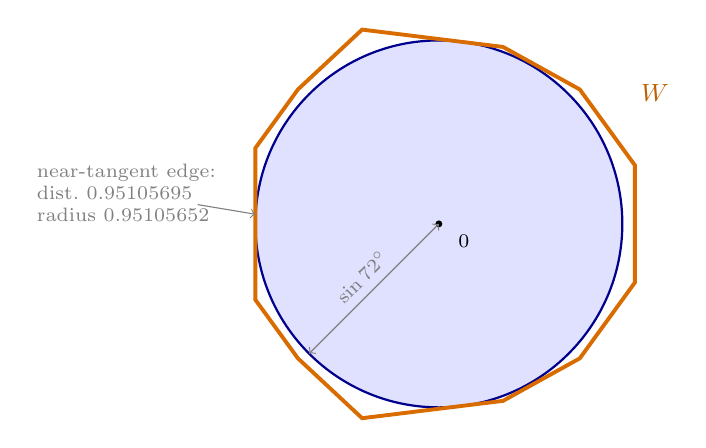
\begin{tikzpicture}[scale=2.45]
% disk
\fill[blue!12] (0,0) circle (0.9510565);
\draw[blue!55!black,thick] (0,0) circle (0.9510565);
% W polygon
\draw[line width=1.4pt,orange!85!black]
 (-0.951057,0.393339) -- (-0.951057,-0.393339) -- (-0.730546,-0.696847)
 -- (-0.397906,-1.007149) -- (0.332640,-0.917317) -- (0.730546,-0.696847)
 -- (1.016324,-0.303507) -- (1.016324,0.303507) -- (0.730546,0.696847)
 -- (0.332640,0.917317) -- (-0.397906,1.007149) -- (-0.730546,0.696847)
 -- cycle;
\fill[black] (0,0) circle (0.018);
\node[font=\scriptsize] at (0.13,-0.09) {$0$};
\draw[<->,gray] (0,0) -- node[above,font=\scriptsize,sloped] {$\sin 72^\circ$} (-0.672,-0.672);
\node[orange!75!black,font=\small\bfseries] at (1.12,0.68) {$W$};
\draw[<-,gray] (-0.9511,0.05) -- (-1.25,0.10);
\node[font=\scriptsize,gray,align=left] at (-1.62,0.16)
 {near-tangent edge:\\ dist.\ $0.95105695$\\ radius $0.95105652$};
\end{tikzpicture}
\caption{The proof of Theorem~\ref{thm:gnomon} in one picture: the Minkowski
sum $W=\gp R_{90^\circ}H\oplus R_{-54^\circ}H\oplus R_{-126^\circ}H$
contains the closed disk of radius $2\operatorname{Area}(T)=\sin72^\circ$.
Every edge line of $W$ keeps distance $\ge \sin72^\circ$ from the origin; by
Corollary~\ref{cor:mink} the staple escapes.  Three of the twelve edges are
tangent to the disk to within $5\times10^{-7}$.}
\label{fig:mink}
\end{figure}

\subsection{The twelve inequalities}
For a convex polygon given by a positively oriented vertex cycle
$w_1,\dots,w_{12}$, the inclusion
$\overline D(0,\rho)\subseteq W$ is equivalent to: (i) all consecutive
cross products $(w_{k+1}-w_k)\times(w_{k+2}-w_{k+1})>0$ (convexity),
(ii) $w_k\times w_{k+1}>0$ for all $k$ (the origin lies inside), and
(iii) for every edge,
\[
\bigl(w_k\times w_{k+1}\bigr)^2\;\ge\;\rho^2\,\lvert w_{k+1}-w_k\rvert^2 ,
\]
i.e., every edge line keeps distance at least $\rho$ from the origin.
Here $\rho^2=\tfrac{5+\sqrt5}{8}$ and all $w_k$ are explicit vectors
with entries in $\Q(\sqrt5,\sqrt{10-2\sqrt5}\,)$, so each of
(i)--(iii) is the sign of an element of that field. Table~\ref{tab:edges}
lists the distances and the certificate values
$D_k=(w_k\times w_{k+1})^2-\rho^2|w_{k+1}-w_k|^2$; by the axial symmetry
of $W$ only seven are distinct. All are strictly positive, with minimum
margin $D=5.13\times10^{-7}$.

The ancillary file \texttt{tight\_staple\_proof.py} constructs these field
elements symbolically and asks SymPy for their exact algebraic signs; decimal
evaluation is used only for the displayed values.  It also verifies exactly
that all $64$ candidate vertex sums lie on or inside every edge half-plane,
so the cycle of Table~\ref{tab:edges} is indeed the boundary of $W$.  Thus
the disk is contained in $W$, and Corollary~\ref{cor:mink} proves that $S$
escapes $T$.

\begin{table}[t]
\centering
\begin{tabular}{@{}lccc@{}}
\toprule
edge of $W$ & multiplicity & distance to $0$ & certificate $D_k$ \\
\midrule
left vertical & 1 & $0.951056952$ & $+5.131\times10^{-7}$ \\
$(-0.951,-0.393)\!\to\!(-0.731,-0.697)$ & 2 & $1.000620318$ & $+1.361\times10^{-2}$ \\
$(-0.731,-0.697)\!\to\!(-0.398,-1.007)$ & 2 & $1.007883096$ & $+2.304\times10^{-2}$ \\
$(-0.398,-1.007)\!\to\!(0.333,-0.917)$ & 2 & $0.951057083$ & $+5.837\times10^{-7}$ \\
$(0.333,-0.917)\!\to\!(0.731,-0.697)$ & 2 & $0.963597925$ & $+4.969\times10^{-3}$ \\
$(0.731,-0.697)\!\to\!(1.016,-0.304)$ & 2 & $1.000620318$ & $+2.287\times10^{-2}$ \\
right vertical & 1 & $1.016323686$ & $+4.731\times10^{-2}$ \\
\midrule
\multicolumn{3}{r}{disk radius $\sin72^\circ$} & $0.9510565$ \\
\bottomrule
\end{tabular}
\medskip
\caption{The distance certificates for the twelve edges of $W$
(mirror-symmetric edges listed once). $D_k>0$ is the exact inequality
(iii); decimals are $60$-digit evaluations truncated for display.}
\label{tab:edges}
\end{table}

\subsection{Length comparisons}
With $t=\tan36^\circ=\sqrt{10-2\sqrt5}/(1+\sqrt5)$:
\[
\begin{array}{llll}
\text{staple (Thm.~\ref{thm:gnomon}):} &
\dfrac{3751558+2\sqrt{20693661817348}}{10^7}
 & =1.2849615\ldots \\[2pt]
\text{square path \cite{ward2008}:} & \dfrac{3\gp\,t}{t+2} & =1.2934739\ldots
 & (+8.512\times10^{-3})\\[6pt]
\text{scaled caliper \cite{zalgaller1961}:} & \zeta\sin36^\circ & =1.3391462\ldots
 & (+5.418\times10^{-2})\\[2pt]
\text{zee \cite{movshovich2012}:} & \dfrac{3\gp\sqrt5}{\sqrt{50+2\sqrt5}} & =1.4706411\ldots
 & (+1.857\times10^{-1})\\[6pt]
\text{diameter:} & \gp & =1.6180340\ldots & (+3.331\times10^{-1})
\end{array}
\]
All five are explicit algebraic numbers except $\zeta$, for which the
directed evaluation $\zeta>2.2782916$ of its published closed form suffices.
This completes the proof of Theorem~\ref{thm:gnomon}. \qed

\begin{remark}
At $\beta=36^\circ$ the base-aligned construction gives the valid square
path in the table.  The leg-aligned value $3s_B=1.2624233\ldots$ is smaller,
but it is not an escape bound there: that square fits strictly inside $T$
(with clearance $6.3\times10^{-3}$), illustrating why
Section~\ref{sec:interval} uses inscribed squares only as \emph{lower}
bounds for escaping square paths.
\end{remark}

\begin{proof}[Proof of Corollary~\ref{cor:bracket}]
Inside $T$ place the isosceles triangle with base angle $45^\circ$, with its
base on the base of $T$ and its apex at the apex of $T$.  Its height is
$h=\sin36^\circ$ and its legs have length $\sqrt2h$.  The escape length of a
unit-leg $45^\circ$ triangle is $3/\sqrt5$ by
\cite{coultonmovshovich2006,movshovich2012}.  Monotonicity under inclusion
and scaling therefore give
\[
 \ell(T)\ge \sqrt2h\,\frac3{\sqrt5}
 =\frac6{\sqrt{10}}\sin36^\circ
 =\frac3{10}\sqrt{25-5\sqrt5}.
\]
The upper bound is Theorem~\ref{thm:gnomon}.
\end{proof}

\section{Numerical discovery and conjectural context}\label{sec:numerics}

\emph{Everything in this section is numerical evidence.}  It is included to
explain how the exact witnesses were found and to identify plausible next
questions.  It is not used in Theorems~\ref{thm:interval}
or~\ref{thm:gnomon}.  In particular, a stationary point within the staple
family is not a proof of optimality, either within that family or among all
escape paths.

For a symmetric staple at the gnomon, numerical constrained optimization
suggests a Karush--Kuhn--Tucker stationary point at
\[
a=0.2430970\ldots,\quad b=0.1875777\ldots,\quad c=0.4515020\ldots,\quad
L=1.2849609182\ldots,
\]
at which one self-symmetric edge and one mirror pair of edges of $W$ are
tangent to the disk.  The rational witness of Theorem~\ref{thm:gnomon} is a
nearby rational point on the feasible side, only $6.16\times10^{-7}$ longer;
the exact disk-containment check, not the stationarity computation, is what
makes it a theorem.  Along the family, the tangency pattern changes twice
near $\beta\approx38.9^\circ$ --- the two interior breakpoints of the
construction in Section~\ref{sec:interval}.

Continuation of the same stationary branch suggests crossings with the
scaled caliper at $\beta\approx31.05^\circ$ and with the zee at
$\beta\approx42.28^\circ$ (the two dots in Figure~\ref{fig:curves}); the
latter agrees strikingly with Gibbs's Monte-Carlo estimate $42.3^\circ$
\cite{gibbs2016}.  These are crossings between three specified candidate
families, not proven phase boundaries of the unrestricted problem; what is
proved is the slightly smaller interval of Corollary~\ref{cor:trio}.  The
wider numerical search also produces nonpolygonal-looking hybrids between
the staple and caliper regimes, at apex angles roughly
$110^\circ$--$118^\circ$; these may be closer to Ward's proposed
``Zalgalloids'', and turning them into exact objects is a natural next
problem.

\section{Conclusion}

The contribution of this paper is a new, exactly certified upper bound for
the escape length of isosceles triangles on the interval
$[31.07^\circ,42.16^\circ]$ of base angles: an explicit trapezoidal family
that removes Ward's square path from the frontier everywhere and beats all
four of his comparison families on $[31.50^\circ,42.16^\circ]$, together
with a finite-certificate method that replaces the continuum of placements
by polygon arithmetic.  No optimality is claimed; the gap in
Corollary~\ref{cor:bracket} remains substantial, and determining whether the
stationary staple, a nearby hybrid, or an entirely different path is optimal
is open.

\subsection*{Ancillary files}
\begin{itemize}
\item \path{tight_staple_proof.py} verifies Theorem~\ref{thm:gnomon}: it
reconstructs $W$, determines the exact algebraic signs in
Table~\ref{tab:edges}, and checks the length comparisons.
\item \path{interval_construction.json} lists the exact rational coefficients
of the staple family $S(u)$.
\item \path{interval_certificate.py} verifies all $116$ Sturm certificates
of Theorem~\ref{thm:interval} and Corollary~\ref{cor:trio}.
\end{itemize}

\begin{thebibliography}{99}

\bibitem{adhikaripitman1989}
A.~Adhikari and J.~Pitman,
\emph{The shortest planar arc of width 1},
Amer. Math. Monthly \textbf{96} (1989), 309--327.

\bibitem{bellman1956}
R.~Bellman,
\emph{Minimization problem},
Bull. Amer. Math. Soc. \textbf{62} (1956), 270.

\bibitem{besicovitch1965}
A.~S. Besicovitch,
\emph{On arcs that cannot be covered by an open equilateral triangle of side 1},
Math. Gazette \textbf{49} (1965), 286--288.

\bibitem{chan2003}
T.~M. Chan, A.~Golynski, A.~L\'opez-Ortiz and C.-G. Quimper,
\emph{Curves of width one and the river shore problem},
Proc. 15th Canad. Conf. Comput. Geom. (CCCG), 2003, 73--75.

\bibitem{coultonmovshovich2006}
P.~Coulton and Y.~Movshovich,
\emph{Besicovitch triangles cover unit arcs},
Geom. Dedicata \textbf{123} (2006), 79--88.

\bibitem{deng2025}
Z.~Deng,
\emph{A general solution to Bellman's lost-in-a-forest problem},
arXiv:2412.10686v3 (2025),
\url{https://arxiv.org/abs/2412.10686v3}.

\bibitem{deng2026}
Z.~Deng,
\emph{Proof and more variations of Bellman's lost-in-a-forest problem},
arXiv:2606.13987v2 (2026),
\url{https://arxiv.org/abs/2606.13987}.

\bibitem{finchwetzel2004}
S.~R. Finch and J.~E. Wetzel,
\emph{Lost in a forest},
Amer. Math. Monthly \textbf{111} (2004), 645--654.

\bibitem{gerrietspoole1974}
J.~Gerriets and G.~Poole,
\emph{Convex regions which cover arcs of constant length},
Amer. Math. Monthly \textbf{81} (1974), 36--41.

\bibitem{gibbs2016}
P.~Gibbs,
\emph{Lost in an isosceles triangle},
viXra:1607.0015 (2016).

\bibitem{gross1955}
O.~Gross,
\emph{A search problem due to Bellman},
RAND Corporation, Research Memorandum RM-1603, 1955.

\bibitem{isbell1957}
J.~R. Isbell,
\emph{An optimal search pattern},
Naval Res. Logist. Quart. \textbf{4} (1957), 357--359.

\bibitem{joris1980}
H.~Joris,
\emph{Le chasseur perdu dans la for\^et},
Elem. Math. \textbf{35} (1980), 1--14.

\bibitem{lutwak1998}
E.~Lutwak,
\emph{Containment and circumscribing simplices},
Discrete Comput. Geom. \textbf{19} (1998), 229--235.

\bibitem{movshovich2012}
Y.~Movshovich,
\emph{Besicovitch triangles extended},
Geom. Dedicata \textbf{159} (2012), 99--107.

\bibitem{movshovichwetzel2011}
Y.~Movshovich and J.~E. Wetzel,
\emph{Escape paths of Besicovitch triangles},
J. Combinatorics \textbf{2} (2011), 413--433.

\bibitem{ward2008}
J.~W. Ward,
\emph{Exploring the Bellman forest problem},
manuscript (2008),
\url{http://wardsattic.com/math/BellmanForestProblem/BellmanForestProblem.pdf};
archived at
\url{https://web.archive.org/web/20250216114838/http://wardsattic.com/math/BellmanForestProblem/BellmanForestProblem.pdf}.

\bibitem{weil1974}
W.~Weil,
\emph{Decomposition of convex bodies},
Mathematika \textbf{21} (1974), 19--25.

\bibitem{zalgaller1961}
V.~A. Zalgaller,
\emph{How to get out of the woods? On a problem of Bellman} (Russian),
Matematicheskoe Prosveshchenie \textbf{6} (1961), 191--195.

\end{thebibliography}

\end{document}
